\section{Overview}

gap in system stack

\from{PACT begin}
\paragraph{Motivation PACT}
The overview of our approach is presented in Figure~\ref{fig:highlevel}.
The programmer expresses his problem by writing a \emph{high-level expression} composed of \emph{algorithmic patterns}.
Using a rewrite rule system, we automatically lower this high-level expression into a \emph{low-level expression} consisting of \emph{hardware patterns}.
This rewrite stage explores the algorithmic and optimization choices in the high-level expression.
The generated low-level expression is then fed into our code generator that emits an \emph{OpenCL program}.
This program is finally compiled to machine code by the vendor provided OpenCL compiler.

The biggest advantage of our approach is that there is no analysis or optimizations performed in the code generator.
All optimization decisions are automatically made earlier on in the rule rewriting system.
This results in a clear separation of concern between the high-level patterns used by the programmer and the low-level hardware paradigms that enable performance portability.

\begin{figure}[t]
\centering
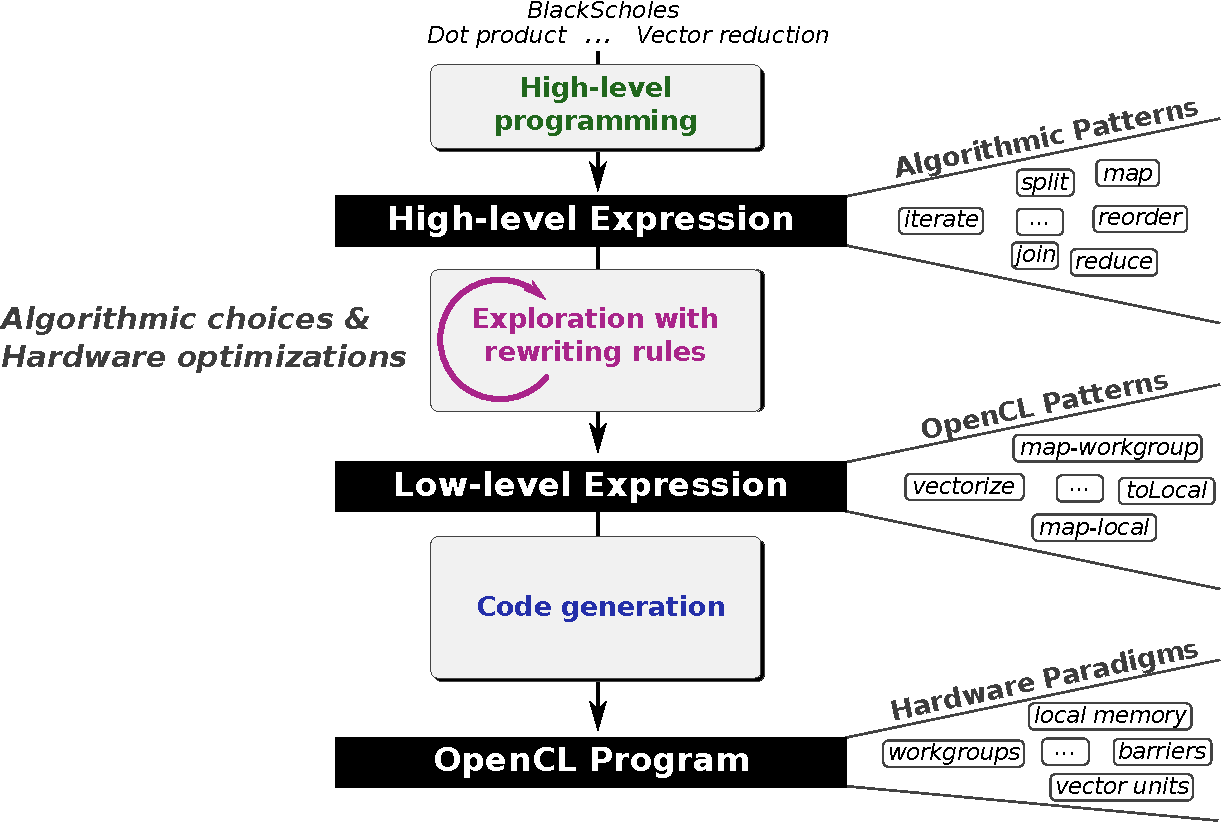
\includegraphics[width=\linewidth]{overviewPatternCodeGeneration}
\vspace{-15pt}
\caption{
The programmer expresses his problem with high-level algorithmic patterns.
A rule rewriting system explores the space of implementations and lower the high-level expression.
Finally, the code generator produces OpenCL code by mapping the low-level hardware patterns directly to the OpenCL programming model representing the hardware paradigms.}
\label{fig:highlevel}
\end{figure}


\subsection{Example}

\begin{figure}[t]
\centering

\begin{subfigure}[b]{.85\linewidth}
\begin{lstlisting}[mathescape,numbers=left]
def mul3(x) = x * 3    // user-defined function
def vectorMul = map(mul3)        // map pattern
\end{lstlisting}
\caption{\textbf{High-level expression} written by the programmer.}
\label{fig:codeex:map}
\end{subfigure}

\vspace{-5pt}
\begin{minipage}{0.1\linewidth}
\vspace{0pt}
\centering
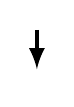
\begin{tikzpicture}[ultra thick]
 \draw [black,   -latex      ] (0,0.5) -- (0,0) node [] {};
\end{tikzpicture}
\end{minipage}
\begin{minipage}{0.25\linewidth}
\vspace{-5pt}
\centering
\textbf{rewrite rules}
\end{minipage}
\begin{minipage}{0.1\linewidth}
\vspace{0pt}
\centering
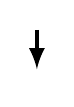
\begin{tikzpicture}[ultra thick]
 \draw [black,   -latex      ] (0,0.5) -- (0,0) node [] {};
\end{tikzpicture}
\end{minipage}

\begin{subfigure}[b]{\linewidth}
\centering
\begin{minipage}{.85\linewidth}
\begin{lstlisting}[mathescape,numbers=left]
def mul3(x) = x * 3
def vectorMul = join $\circ$ map-workgroup(
                  join $\circ$ map-local(
                    vectorize-4(mul3)
                  ) $\circ$ split-4
                ) $\circ$ split-1024
\end{lstlisting}
\end{minipage}
\caption{\textbf{Low-level expression} automatically derived using rewrite rules.}
\label{fig:codeex:impl}
\end{subfigure}

\vspace{-5pt}
\begin{minipage}{0.1\linewidth}
\vspace{0pt}
\centering
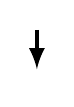
\begin{tikzpicture}[ultra thick]
 \draw [black,   -latex      ] (0,0.5) -- (0,0) node [] {};
\end{tikzpicture}
\end{minipage}
\begin{minipage}{0.26\linewidth}
\vspace{-5pt}
\centering
\textbf{code generator}
\end{minipage}
\begin{minipage}{0.1\linewidth}
\vspace{0pt}
\centering
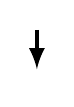
\begin{tikzpicture}[ultra thick]
 \draw [black,   -latex      ] (0,0.5) -- (0,0) node [] {};
\end{tikzpicture}
\end{minipage}

\begin{subfigure}[b]{\linewidth}
\centering
\begin{minipage}{.85\textwidth}
\begin{lstlisting}[mathescape,numbers=left]
int4 mul3(int4 x) { return x * 3; }
kernel map_mul3(global int* in,out, int len) {
  // division into workgroup by chuncks of 1024
  for (int i=get_group_id; i < len/1024;
       i+=get_num_groups) {
    global int* grp_in  = in+(i*1024);
    global int* grp_out = out+(i*1024);
    // division into threads by chunks of 4
    for (int j=get_local_id; j < 1024/4;
         j+=get_local_size) {
      global int* lcl_in  = grp_in+(j*4);
      global int* lcl_out = grp_out+(j*4);
      // vectorization with vector width of 4
      global int4* in_vec4 = (int4*) lcl_in;
      global int4* out_vec4 = (int4*) lcl_out;
      *out_vec4 = mul3(*in_vec4);      
} } }  
\end{lstlisting}
\end{minipage}
\caption{\textbf{OpenCL program} automatically produced by our code generator.}
\label{fig:codeex:ocl}
\end{subfigure}

\caption{Pseudo-code representing a vector scaling program.
The user simply maps the \texttt{mul3} function over the elements of the input array~(\subref{fig:codeex:map}).
This high-level expression is automatically transformed into a low-level expression~(\subref{fig:codeex:impl}) using rewrite rules.
Finally, our code generator turns the low-level expression into an OpenCL program~(\subref{fig:codeex:ocl}).}
\label{fig:codeex}
\end{figure}

We now present the advantages of our approach with a simple vector scaling example shown in Figure~\ref{fig:codeex}.
The user expresses the computation by writing a high-level expression using our \pat{map} algorithmic pattern as shown in Figure~\ref{fig:codeex:map}.
This coding style is similar to functional and dataflow programming.

Our technique first rewrites automatically the user provided high-level expression into something closer to the OpenCL programming model.
This is achieved by applying the rewrite rules presented later in Section~\ref{rules}.
Figure~\ref{fig:codeex:impl} shows one possible derivation of the original high-level map expression where the $\circ$ operator represents function composition, \ie $f \circ g(x) = f(g(x))$.
Starting from the last line, we first split the input into chunks of 1024 elements.
Each chunk is mapped onto a workgroup with the \pat{map-workgroup} low-level pattern (line~2).
Within a workgroup (lines~3--5), we further split the elements into chunks of 4 (line~5), each mapped to a local thread via the \pat{map-local} low-level pattern (line~3).
Each local thread is responsible for processing 4 elements.
Finally, the \pat{vectorize-4} pattern (line~4) implies that the user defined function \texttt{mul3} is vectorized.
The exact meaning of our patterns will be given later in Section~\ref{pattern}.

The last step consists of traversing the low-level expression and generating OpenCL code (see Figure~\ref{fig:codeex:ocl}) for each low-level pattern encountered.
The two map patterns generate the for loops (line~4--5 and~9--10) that iterate over the input array assigning work to the workgroups and local threads.
The information of how many chunks each workgroup and thread processes comes from the corresponding \pat{split}.
In line~16 the vectorized version of the user defined \texttt{mul3} function (defined in line~1) is finally applied to the input array.

To summarize, our approach is able to automatically generate OpenCL code starting from a high-level representation of a program.
This is achieved by automatically lowering the high-level expression into a low-level form suitable for code generation.
The next two sections present our high-level and low-level patterns, the code generation mechanism and the rewrite rules in more details.
\from{PACT end}

\from{PPoPP begin}
\paragraph{Motivation PPoPP}
The overview of our approach is presented in Figure~\ref{fig:highlevel}.
The programmer writes a \emph{high-level expression} composed of \emph{algorithmic patterns}.
Using a rewrite rule system, we systematically lower this high-level expression into a \emph{low-level expression} consisting of \emph{OpenCL patterns}.
In this rewrite stage algorithmic and optimization choices in the high-level expression can be explored.
The generated low-level expression is then fed into our code generator that emits an \emph{OpenCL program}.
This program is finally compiled to machine code by the vendor provided OpenCL compiler.

% One big advantage of our approach is that there is no analysis or optimizations performed in the code generator.
% All optimization decisions are automatically made earlier on in the rule rewriting system.
% This results in a clear separation of concern between the high-level patterns used by the programmer and the low-level hardware paradigms that enable performance portability.

\begin{figure}[t]
\centering
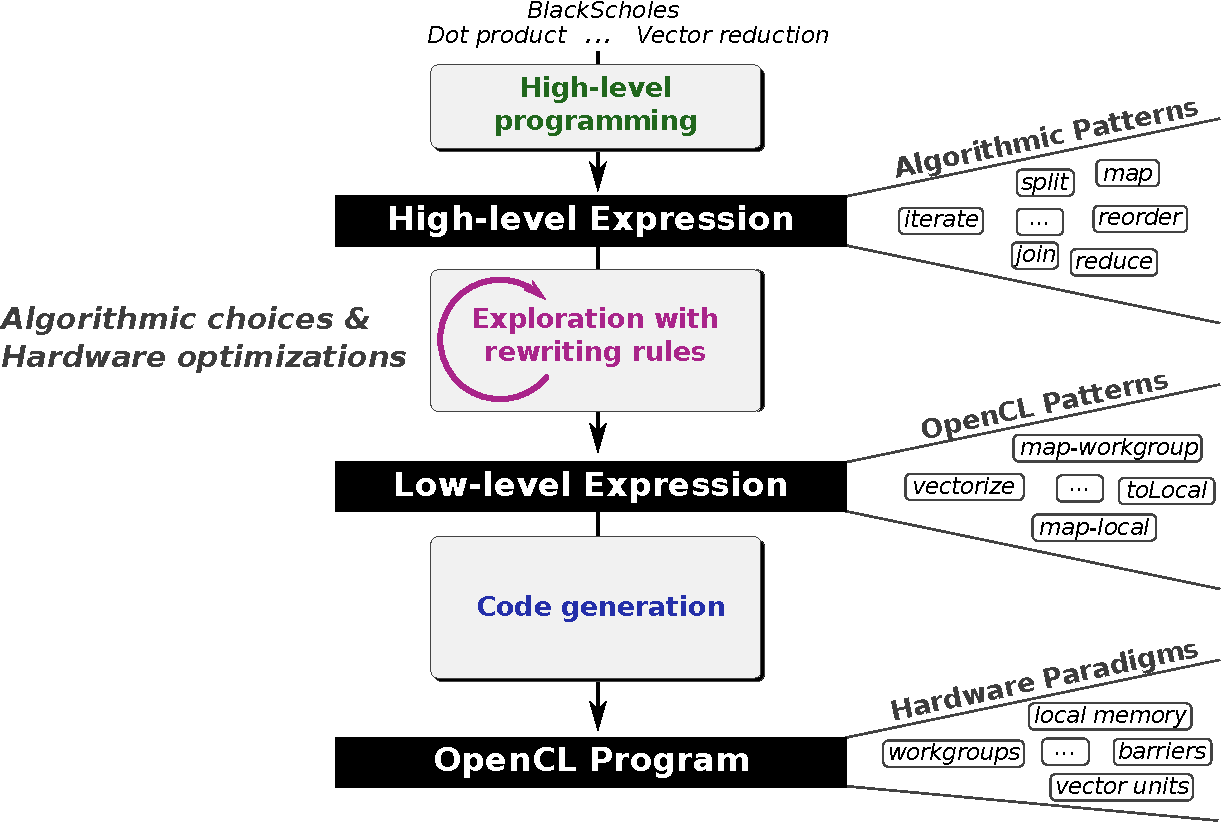
\includegraphics[width=\linewidth]{overviewPatternCodeGeneration}
\vspace{-19pt}
\caption{
Overview of our system.
The programmer expresses the problem with high-level algorithmic patterns.
These are systematically transformed into low-level OpenCL patterns using a rule rewriting system.
OpenCL code is generated by mapping the low-level patterns directly to the OpenCL programming model representing hardware paradigms.
\vspace{-1em}}
\label{fig:highlevel}
\end{figure}





% \subsection{Example}

\begin{figure}[t]
\centering

\begin{subfigure}[b]{.85\linewidth}%{0.7\linewidth}
\begin{lstlisting}[mathescape,numbers=left]
def mul3(x) = x * 3    // user-defined function
def vectorScal = map(mul3)       // map pattern
\end{lstlisting}
\caption{\textbf{High-level expression} written by the programmer.}
\label{fig:codeex:map}
\end{subfigure}

\vspace{-10pt}
\begin{minipage}{0.1\linewidth}
\vspace{0pt}
\centering
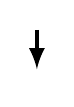
\begin{tikzpicture}[ultra thick]
 \draw [black,   -latex      ] (0,0.5) -- (0,0) node [] {};
\end{tikzpicture}
\end{minipage}
\begin{minipage}{0.25\linewidth}
\vspace{-5pt}
\centering
\textbf{rewrite rules}
\end{minipage}
\begin{minipage}{0.1\linewidth}
\vspace{0pt}
\centering
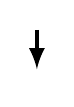
\begin{tikzpicture}[ultra thick]
 \draw [black,   -latex      ] (0,0.5) -- (0,0) node [] {};
\end{tikzpicture}
\end{minipage}

\vspace{0pt}
\begin{subfigure}[b]{\linewidth}
\centering
\begin{minipage}{.85\linewidth}%{0.85\textwidth}
\begin{lstlisting}[mathescape,numbers=left]
def mul3(x) = x * 3
def vectorScal = join $\circ$ map-workgroup(
                  asScalar $\circ$ map-local(
                    vectorize-4(mul3)
                  ) $\circ$ asVector-4
                 ) $\circ$ split-1024
\end{lstlisting}
\end{minipage}
\caption{\textbf{Low-level expression} systematically derived using rewrite rules.}
\label{fig:codeex:impl}
\end{subfigure}

\vspace{-10pt}
\begin{minipage}{0.1\linewidth}
\vspace{0pt}
\centering
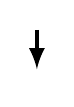
\begin{tikzpicture}[ultra thick]
 \draw [black,   -latex      ] (0,0.5) -- (0,0) node [] {};
\end{tikzpicture}
\end{minipage}
\begin{minipage}{0.26\linewidth}
\vspace{-5pt}
\centering
\textbf{code generator}
\end{minipage}
\begin{minipage}{0.1\linewidth}
\vspace{0pt}
\centering
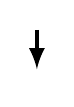
\begin{tikzpicture}[ultra thick]
 \draw [black,   -latex      ] (0,0.5) -- (0,0) node [] {};
\end{tikzpicture}
\end{minipage}

\vspace{0pt}
\begin{subfigure}[b]{\linewidth}
\centering
\begin{minipage}{.85\textwidth}
\begin{lstlisting}[mathescape,numbers=left]
int4 mul3(int4 x) { return x * 3; }
kernel vectorScal(global int* in,out, int len){
 for (int i=get_group_id; i < len/1024;
      i+=get_num_groups) {
  global int* grp_in  = in+(i*1024);
  global int* grp_out = out+(i*1024);
  for (int j=get_local_id; j < 1024/4;
       j+=get_local_size) {
    global int4* in_vec4 =(int4*)grp_in+(j*4);
    global int4* out_vec4=(int4*)grp_out+(j*4);
    *out_vec4 = mul3(*in_vec4);      
} } }  
\end{lstlisting}
\end{minipage}
\caption{\textbf{OpenCL program} produced by our code generator.}
\label{fig:codeex:ocl}
\end{subfigure}
\vspace{-20pt}
\caption{
Pseudo-code representing vector scaling.
The user simply maps the \code{mul3} function over the elements of the input array~(\subref{fig:codeex:map}).
This high-level expression is systematically transformed into a low-level expression~(\subref{fig:codeex:impl}) using rewrite rules.
Finally, our code generator turns the low-level expression into an OpenCL program~(\subref{fig:codeex:ocl}).
}
  \label{fig:codeex}
\end{figure}

We now illustrate the advantages of our approach using a simple vector scaling example shown in Figure~\ref{fig:codeex}.
The user expresses the computation by writing a high-level expression using our \pat{map} algorithmic pattern as shown in Figure~\ref{fig:codeex:map}.
This coding style is similar to functional and dataflow programming.

Our technique first rewrites the user provided high-level expression into something closer to the OpenCL programming model.
This is achieved by applying the rewrite rules presented later in Section~\ref{rules}.
Figure~\ref{fig:codeex:impl} shows one possible derivation of the original high-level expression where the $\circ$ operator represents function composition, \ie $f \circ g(x) = f(g(x))$.
Starting from the last line, we first split the input into chunks of 1024 elements.
Each chunk is mapped onto a group of threads, called \emph{workgroup}, with the \pat{map-workgroup} low-level pattern (line~2).
Within a workgroup (lines~3--5), we vectorize the elements (line~5), each mapped to a local thread inside a workgroup via the \pat{map-local} low-level pattern (line~3).
Each local thread now processes 4 elements, enclosed in a vector type.
Finally, the \pat{vectorize-4} pattern (line~4) implies that the user defined function \code{mul3} is vectorized.
The exact meaning of our patterns will be given later in Section~\ref{pattern}.

The last step consists of traversing the low-level expression and generating OpenCL code for each low-level pattern encountered (Figure~\ref{fig:codeex:ocl}).
The two map patterns generate the for loops (line~3--4 and~7--8) that iterate over the input array assigning work to the workgroups and local threads.
The information of how many chunks each workgroup and thread processes comes from the corresponding \pat{split}.
In line~11 the vectorized version of the user defined \code{mul3} function (defined in line~1) is finally applied to the input array.

To summarize, our approach is able to generate OpenCL code starting from a high-level representation of a program.
This is achieved by systematically lowering the high-level expression into a low-level form suitable for code generation.
The next two sections present our high-level and low-level patterns, the code generation mechanism and the rewrite rules in more details.
\from{PPoPP end}

\from{PLDI begin}
\paragraph{Motivation PLDI}
The overview of our approach is presented in Figure~\ref{fig:highlevel}.
The programmer writes a \emph{high-level expression} composed of \emph{algorithmic patterns}.
Using a rewrite rule system, we lower this high-level expression into a \emph{low-level expression} consisting of \emph{OpenCL patterns}.
In this rewrite stage algorithmic and optimization choices in the high-level expression can be explored.
The generated low-level expression is then fed into our code generator that emits an \emph{OpenCL program} compiled to machine code by the vendor provided OpenCL compiler.

\begin{figure}[t]
\centering
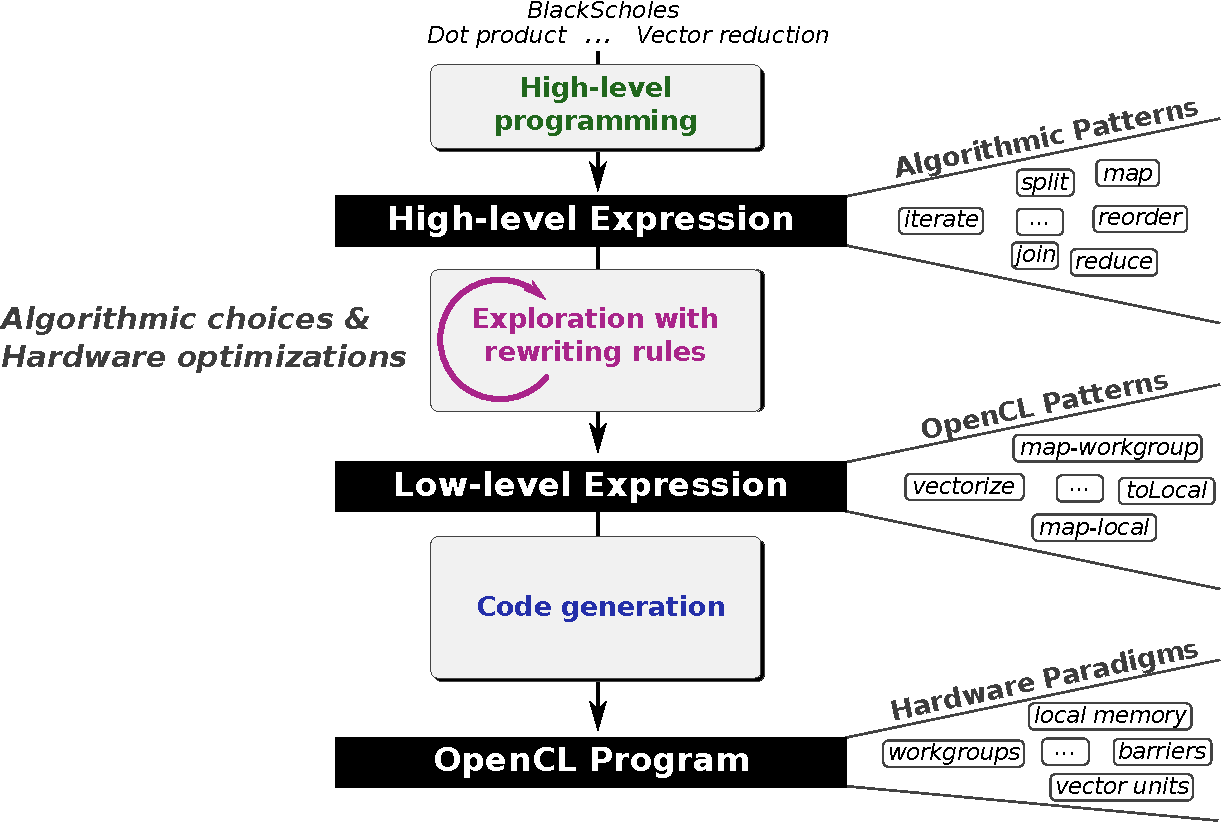
\includegraphics[width=\linewidth]{overviewPatternCodeGeneration}
\vspace{-19pt}
\caption{
Overview of our system.
The programmer expresses the problem with high-level algorithmic patterns.
These are systematically transformed into low-level patterns using a rule rewriting system.
OpenCL code is generated by mapping the low-level patterns directly to the OpenCL programming model representing hardware paradigms.
\vspace{-1em}}
\label{fig:highlevel}
\end{figure}





% \subsection{Example}

\begin{figure}[t]
\centering

\begin{subfigure}[b]{.85\linewidth}%{0.7\linewidth}
\begin{lstlisting}[mathescape,numbers=left]
def mul3(x) = x * 3    // user-defined function
def vectorScal = map(mul3)       // map pattern
\end{lstlisting}
\caption{\textbf{High-level expression} written by the programmer.}
\label{fig:codeex:map}
\end{subfigure}

\vspace{-10pt}
\begin{minipage}{0.1\linewidth}
\vspace{0pt}
\centering
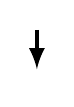
\begin{tikzpicture}[ultra thick]
 \draw [black,   -latex      ] (0,0.5) -- (0,0) node [] {};
\end{tikzpicture}
\end{minipage}
\begin{minipage}{0.25\linewidth}
\vspace{-5pt}
\centering
\textbf{rewrite rules}
\end{minipage}
\begin{minipage}{0.1\linewidth}
\vspace{0pt}
\centering
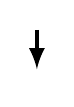
\begin{tikzpicture}[ultra thick]
 \draw [black,   -latex      ] (0,0.5) -- (0,0) node [] {};
\end{tikzpicture}
\end{minipage}

\vspace{-5pt}
\begin{subfigure}[b]{\linewidth}
\centering
\begin{minipage}{.85\linewidth}%{0.85\textwidth}
\begin{lstlisting}[mathescape,numbers=left]
def mul3(x) = x * 3
def vectorScal = join $\circ$ map-workgroup(
                  asScalar $\circ$ map-local(
                    vect-4(mul3)
                  ) $\circ$ asVector-4
                 ) $\circ$ split-1024
\end{lstlisting}
\end{minipage}
\caption{\textbf{Low-level expression} derived using rewrite rules.}
\label{fig:codeex:impl}
\end{subfigure}

\vspace{-5pt}
\begin{minipage}{0.1\linewidth}
\vspace{0pt}
\centering
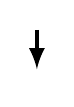
\begin{tikzpicture}[ultra thick]
 \draw [black,   -latex      ] (0,0.5) -- (0,0) node [] {};
\end{tikzpicture}
\end{minipage}
\begin{minipage}{0.26\linewidth}
\vspace{-5pt}
\centering
\textbf{code generator}
\end{minipage}
\begin{minipage}{0.1\linewidth}
\vspace{0pt}
\centering
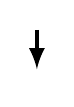
\begin{tikzpicture}[ultra thick]
 \draw [black,   -latex      ] (0,0.5) -- (0,0) node [] {};
\end{tikzpicture}
\end{minipage}

\vspace{0pt}
\begin{subfigure}[b]{\linewidth}
\centering
\begin{minipage}{.85\textwidth}
\begin{lstlisting}[mathescape,numbers=left]
int4 mul3(int4 x) { return x * 3; }
kernel vectorScal(global int* in,out, int len){
 for (int i=get_group_id; i < len/1024;
      i+=get_num_groups) {
  global int* grp_in  = in+(i*1024);
  global int* grp_out = out+(i*1024);
  for (int j=get_local_id; j < 1024/4;
       j+=get_local_size) {
    global int4* in_vec4 =(int4*)grp_in+(j*4);
    global int4* out_vec4=(int4*)grp_out+(j*4);
    *out_vec4 = mul3(*in_vec4);      
} } }  
\end{lstlisting}
\end{minipage}
\caption{\textbf{OpenCL program} produced by our code generator.}
\label{fig:codeex:ocl}
\end{subfigure}
\vspace{-25pt}
\caption{
Pseudo-code representing vector scaling.
The user maps the \code{mul3} function over the input array~(\subref{fig:codeex:map}).
This high-level expression is transformed into a low-level expression~(\subref{fig:codeex:impl}) using rewrite rules.
Finally, our code generator turns the low-level expression into an OpenCL program~(\subref{fig:codeex:ocl}).
}
  \label{fig:codeex}
\end{figure}

We illustrate the advantages of our approach using a simple vector scaling example shown in Figure~\ref{fig:codeex}.
The user expresses the computation by writing a high-level expression using our \pat{map} pattern as shown in Figure~\ref{fig:codeex:map}.
This coding style is similar to functional and dataflow programming.

Our technique first rewrites the high-level expression into something closer to the OpenCL programming model.
This is achieved by applying the rewrite rules presented later in Section~\ref{rules}.
Figure~\ref{fig:codeex:impl} shows one possible derivation of the original high-level expression.
The $\circ$ operator represents sequential function composition. %, \ie $f \circ g(x) = f(g(x))$.
Starting from the last line, the input is split into chunks of 1024 elements.
Each chunk is mapped onto a group of threads, called \emph{workgroup}, with the \pat{map-workgroup} low-level pattern (line~2).
Within a workgroup (lines~3--5), we vectorize the elements (line~5), each mapped to a local thread inside a workgroup via the \pat{map-local} pattern (line~3).
Each local thread now processes 4 elements, enclosed in a vector type.
Finally, the \pat{vect-4} pattern (line~4) vectorizes the user defined function \code{mul3}.
The exact meaning of our patterns will be given later in Section~\ref{pattern}.

The last step consists of traversing the low-level expression and generating OpenCL code for each low-level pattern encountered (Figure~\ref{fig:codeex:ocl}).
The two map patterns generate the for-loops (line~3--4 and~7--8) that iterate over the input array assigning work to the workgroups and local threads.
The information of how many chunks each workgroup and thread processes comes from the corresponding \pat{split}.
In line~11 the vectorized version of the user defined \code{mul3} function (defined in line~1) is finally applied to the input array.

To summarize, our approach is able to generate OpenCL code starting from a high-level program representation. % of a program.
This is achieved by systematically lowering the high-level expression into a low-level form suitable for code generation.
The next two sections present our high-level and low-level patterns, the code generation mechanism and the rewrite rules. % in more details.
\from{PLDI end}

